%        File: HW02.tex
%     Created: 一 7月 09 08:00 下午 2018 C
% Last Change: 一 7月 09 08:00 下午 2018 C
%
\documentclass[UTF8,noindent]{ctexart}
\usepackage[a4paper,left=2.0cm,right=2.0cm,top=2.0cm,bottom=2.0cm]{geometry}
\usepackage{hyperref}
\usepackage{url}
\usepackage{graphicx}
\usepackage{amsmath}
\usepackage{amssymb}
\usepackage{enumitem}
\usepackage{tikz}
\usepackage{float}
\usepackage{forest}
\usepackage{pgf}
\usetikzlibrary{graphs}
\usetikzlibrary{arrows,automata}
\usepackage{listings}
\usepackage{xcolor}
\lstset{language = c,numbers=left, showstringspaces = false, keywordstyle= \color{ blue!70 },commentstyle=\color{red!50!green!50!blue!50}, frame=shadowbox, rulesepcolor= \color{ red!20!green!20!blue!20 } 
} 
\usetikzlibrary{graphs}
\title{$Chapter\ 2-HW02$}
\author{$2015K8009929049$\ 冯吕}
\date{\today}
\begin{document}
\maketitle
\zihao{5}
\CJKfamily{zhsong}
$1.$解:

$1)$令$\lambda_1 = (a|b|..|d|f|..|h|j|..|n|p|..|t|v|..|z), \lambda_2 = (b|c|..|h|j|..|n|p|..|t|v|..|z), \lambda_3 = (b|c|..|d|f|..|n|p|..|t|v|..z), \lambda_4 = (b|c|..|d|f|..|h|j|..|t|v|..|z), \lambda_5 = (b|c|..|d|f|..|h|j|..|n|p|..|z)$,则对应的$DFA$如下:
%\[\lambda_1^*a+\lambda_1^*\lambda_2^*e+\lambda_3^*\lambda_3^*i+\lambda_3^*\lambda_4*o+\lambda_4^*\lambda_5^*u+\lambda_5^*\]
\begin{center}
  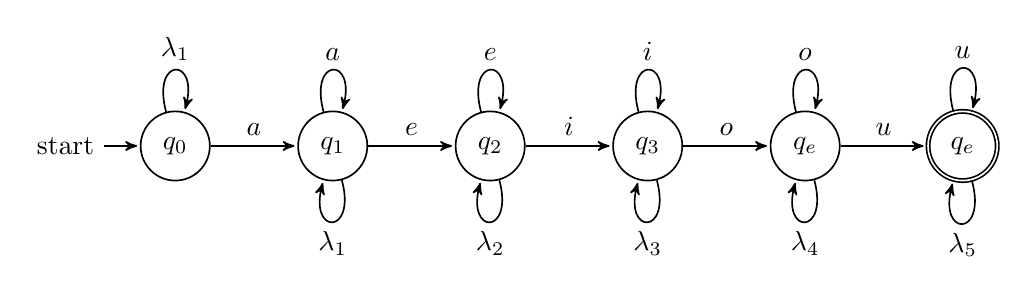
\begin{tikzpicture}[->,>=stealth',shorten >=1pt,auto,node distance=2cm,semithick]
	\node[initial, state] (A)    {$q_0$};
	\node [state] (B) [right of = A] {$q_1$};
	\node [state] (C) [right of = B] {$q_2$};
	\node [state] (D) [right of = C]   {$q_3$};
	\node [state] (E) [right of = D] {$q_e$};
	\node [state, accepting] (F) [right of = E] {$q_e$};
	\path (A) edge [loop above] node {$\lambda_1$} (A);
	\path (A) edge node {$a$} (B);

	\path (B) edge [loop above] node {$a $} (B);
	\path (B) edge [loop below] node {$ \lambda_1$} (B);
	\path (B) edge node {$e$} (C);

	\path (C) edge [loop above] node {$e $} (C);
	\path (C) edge [loop below] node {$ \lambda_2$} (C);
	\path (C) edge node {$i$} (D);

	\path (D) edge [loop above] node {$i$} (D);
	\path (D) edge [loop below] node {$\lambda_3$} (D);
	\path (D) edge node {$o$} (E);

	\path (E) edge [loop above] node {$o$} (E);
	\path (E) edge [loop below] node {$ \lambda_4$} (E);
	\path (E) edge node {$u$} (F);

	\path (F) edge [loop above] node {$u$} (F);
	\path (F) edge [loop below] node {$ \lambda_5$} (F);
	%\path (E) edge node {$\epsilon$} (B);
  \end{tikzpicture}
\end{center}

$2)$由$a,b$组成不含子串$abb$的语言对应的正则表达式为$b^*(ab?)^*$,经转化和化简得识别它的$DFA$如下:
\begin{center}
  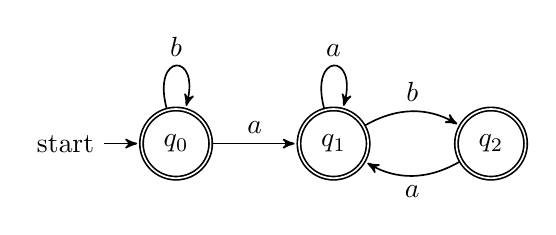
\begin{tikzpicture}[->,>=stealth',shorten >=1pt,auto,node distance=2cm,semithick]
	\node [initial , state, accepting] (A)  {$q_0$};
	\node [state, accepting] (B) [right of = A] {$q_1$};
	\node [state, accepting] (C) [right of = B] {$q_2$};

  \path (A) edge node {$a$} (B);
  \path (A) edge[loop above] node {$b$} (A);
  \path (B) edge[loop above] node {$a$} (B);
  \path (B) edge [bend left] node {$b$} (C);
  \path (C) edge [bend left] node {$a$} (B);

  \end{tikzpicture}
\end{center}

$2.$解:图$3.29$中的$NFA$包含$4$个状态,其中$F=\{3\}$。
\begin{itemize}
  \item $(1)$初始:$S = \{0\}; c = nextChar() = a$;
  \item $(2) c!= EOF\Rightarrow S = \epsilon-closure(move(S, a)) = \{0, 1\}; c = nextChar() = a$;
  \item $(3) c!= EOF \Rightarrow S = \epsilon-closure(move(S,a)) = \{0, 1, 2\}; c = nextChar() = b$;
  \item $(4) c != EOF\Rightarrow S = \epsilon-closure(move(S,b)) = \{0, 1, 2, 3\}; c = nextChar() = b$;
  \item $(4) c != EOF\Rightarrow S = \epsilon-closure(move(S, b)) = \{0, 1, 2, 3\}; c = nextChar() = EOF$;
  \item $(5) c == EOF \Rightarrow S\cap F = \{3\} \neq \emptyset$;
\end{itemize}
所以,该$NFA$能够接受字符串$aabb$。

$3.$解:

$1)$根据算法$3.23, 3.20$转化并化简得$((\epsilon|a)b^*)^*$对应的$DFA$如下:
\begin{center}
  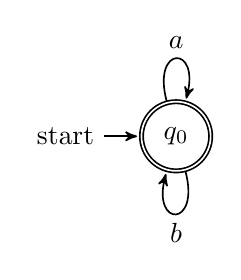
\begin{tikzpicture}[->,>=stealth',shorten >=1pt,auto,node distance=4cm,semithick]
	\node [initial,accepting , state] (A)  {$q_0$};
	%\node [state, accepting] (B) [above right of = A] {$q_1$};
	%\node [state, accepting] (C) [below right of = A] {$q_2$};

  %\path (A) edge node {$a$} (B);
  %\path (A) edge node[below] {$b$} (C);
  %\path (B) edge [bend left] node {$\epsilon$} (A);

  %\path (B) edge node {$b$} (C);
  %\path (C) edge[bend left] node {$a$} (B);
  \path (A) edge[loop above] node {$a$} (A);
  \path (A) edge[loop below] node {$b$} (A);
  \end{tikzpicture}
\end{center}

$2)(a|b)^*abb(a|b)^*$对应的$DFA$(经化简)如下:
\begin{center}
  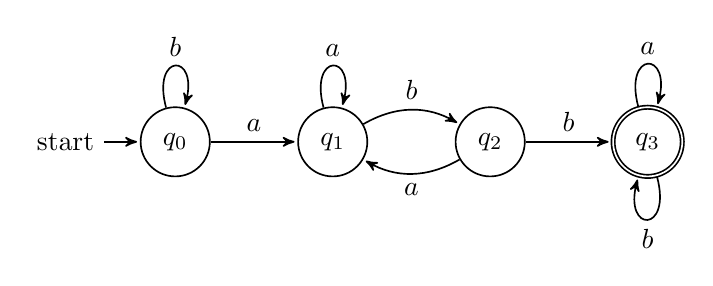
\begin{tikzpicture}[->,>=stealth',shorten >=1pt,auto,node distance=2cm,semithick]
	\node [initial , state] (A)  {$q_0$};
	\node [state ] (B) [right of = A] {$q_1$};
  \node [state] (C) [right of = B] {$q_2$};
  \node [state, accepting] (D) [right of = C] {$q_3$};

  \path (A) edge node {$a$} (B);
  \path (A) edge[loop above] node {$b$} (A);
  \path (B) edge[loop above] node {$a$} (B);

  \path (B) edge[bend left] node {$b$} (C);
  \path (C) edge[bend left] node {$a$} (B);
  \path (C) edge node {$b$} (D);
  \path (D) edge[loop below] node {$b$} (D);
  \path (D) edge[loop above] node {$a$} (D);
  \end{tikzpicture}
\end{center}


\end{document}


